
	\section{Genetic Analysis of Schizophrenia}
	\subsection{Genetic Architecture of Schizophrenia}
	\begin{wrapfigure}{R}{8cm}
		\centering
		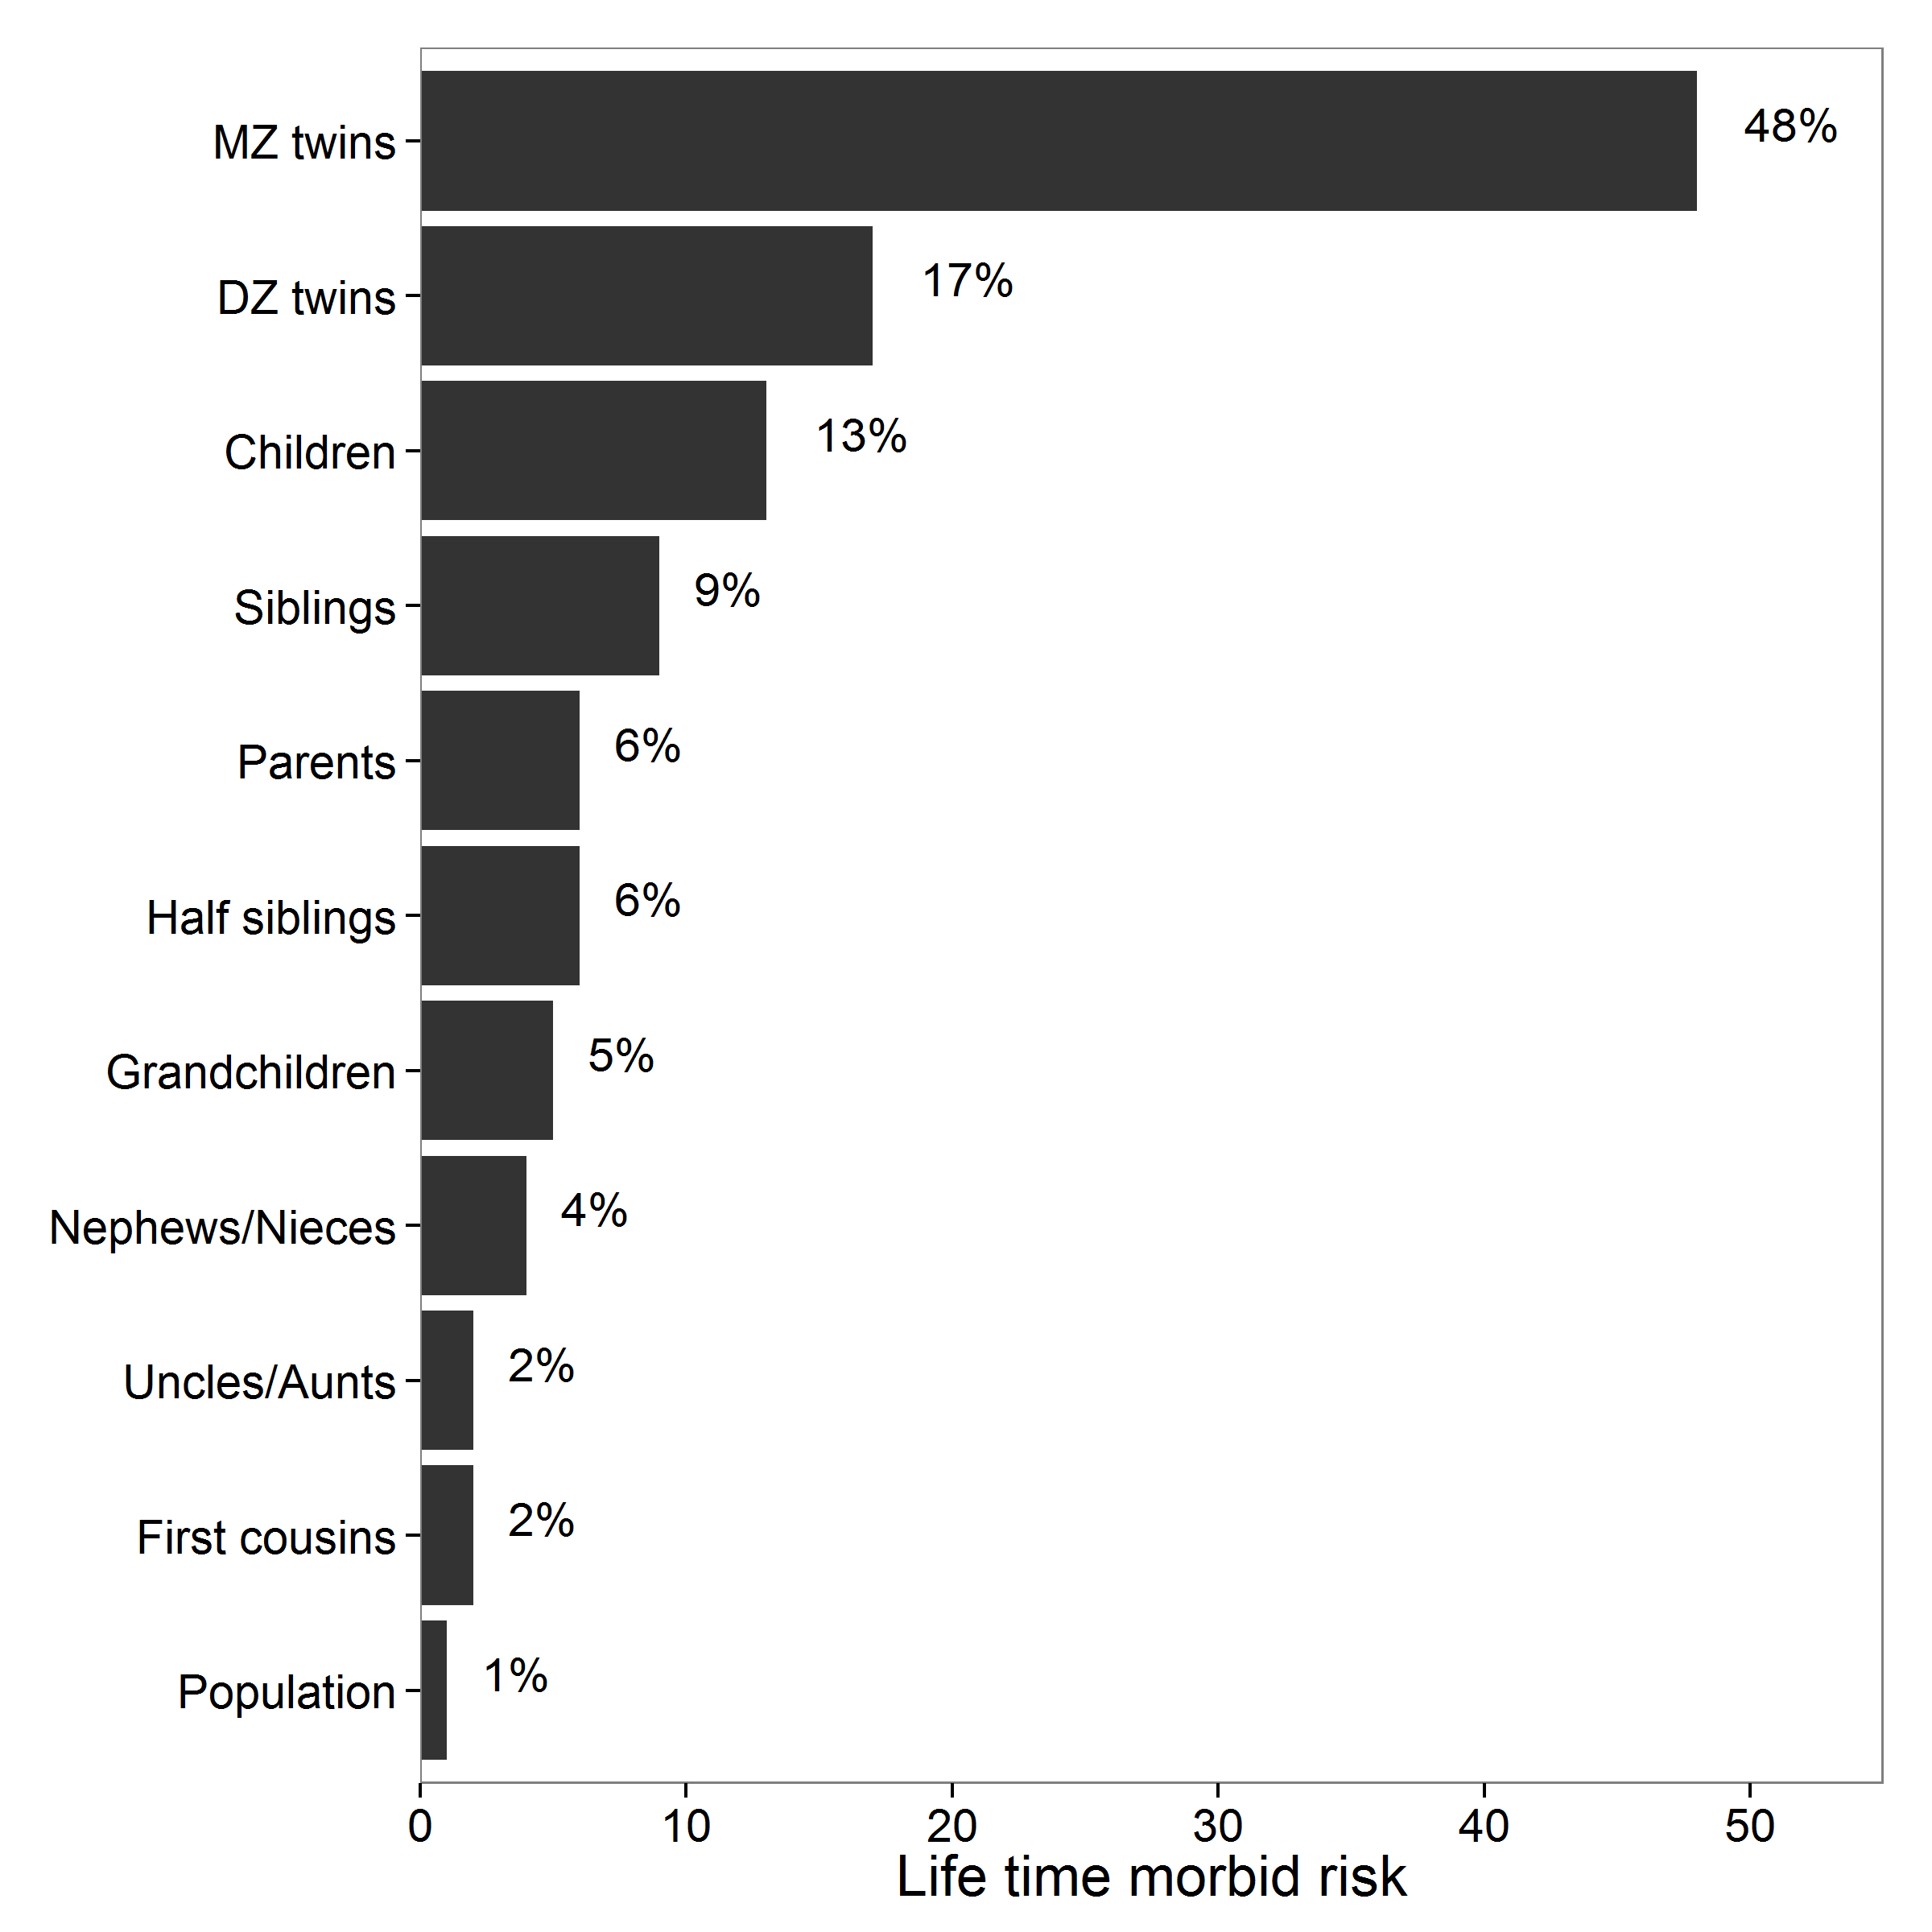
\includegraphics[width=0.5\textwidth]{figure/lifeTimeMorbidRisk.png}
		\caption[Lifetime morbid risks of \glng{scz} in various classes of relatives of a proband]{Lifetime morbid risks of \glng{scz} in various classes of relatives of a proband.
			It was noted that the morbid risk of monozygotic (MZ) twins were only $48\%$, much lower than one would expect if \glng{scz} follows a Mendelian pattern.
			Reproduced with permission from journal\citep{Riley2006}. \label{fig:lifeMRscz}}
	\end{wrapfigure}
	Studies on estimation of heritability of \glng{scz} strongly support \glng{scz} as a genetic disorder.
	However, little was known about the mechanism of \glng{scz} nor the genetic architecture of the disorder. 
	All data from adoption studies, twin studies and family studies shown that \glng{scz} does not follow the Mendelian framework\citep{Gottesman01071967,Gottesman1982}.
	Specifically, shall \glng{scz} be a Mendelian disorder, then we would expect all \gls{mz} siblings of the proband to also suffer from \glng{scz}.
	However, the life time morbid risk of monozyogitc twins were only $48\%$(\cref{fig:lifeMRscz})\citep{gottesman1991schizophrenia}, making it unlikely for \glng{scz} to follow a Mendelian pattern.
	
	Based on these observations, \cite{Gottesman1967} proposed that \glng{scz} follows a polygenic model where disease phenotype were determined by the additive effects from multiple genes.
	Thus, \glng{scz} is a complex genetic disorder with complicated pattern of inheritance. 
	Their hypothesis was supported by the calculation of \cite{Risch1990a} by taking into account of different inheritance model and the life time morbid risk observed in relatives of affected individuals.
	
	Another interesting conclusion from the calculation of \citet{Risch1990a} was the effect size of individual locus. 
	By comparing the observed life time morbid risk and the calculated risk from different models, \citeauthor{Risch1990a} 	suggested that genetic models with a single locus with risk of 3.0 and with all other loci of small effect or models with two or three loci with risk of 2.0 were most consistent with the observed life time morbid risk of \glng{scz}.	\citep{Risch1990}.
	
	\citeauthor{Risch1990a}'s calculation provided an explanation for the early inconsistent findings of linkage studies in \glng{scz}\citep{Harrison2005}.
	As linkage studies were aimed to identify genetic variation of large effect size they failed to capture genetic loci with small effect size.
	It was therefore tempting to suggest that \glng{scz} only follows the ``common disease-common variant'' model, which stated that \glng{scz} should be mediated by large amount of common variants such as \glng{SNP}, each carries a small effect size.
	
	However, another possible hypothesis was that the variation mediating \glng{scz} were rare, therefore require a large sample size to detect. 
	The inconsistent results of the early linkage studies might be due to the inadequate sample size. 
	This lead to some researchers suggesting the ``common disease-rare variant'' hypothesis, which propose that \glng{scz} was mediated by a small amount of rare variants, each with a large effect size\citep{McClellan2007}.
	
	Nevertheless, success in genetic research of \glng{scz} remains limited.
	Only until the initiation of Human Genome Project and the technological advance resulted from it that does genetic research of \glng{scz} entered an era of success.

	\subsection{The Human Genome Project and HapMap Project}
	\glsreset{SNP}
	\glsreset{LD}
	In 1990, the Human genome project was initiated, aiming at constructing the first physical map of the human genome at per nucleotide resolution\citep{Lander2001}.
	The completion of the human genome project has opened up a new era of genetic research, allowing researchers to identify \glspl{SNP} on the human genome, which is one of the major source of genetic variation.
	
	Soon after the completion of the human genome project, the HapMap Project was initiated\citep{Consortium2005}, aiming to provide a genome-wide database of common human sequence variation such as \glspl{SNP} with \gls{maf} $\ge0.05$.
	More importantly was that the HapMap Project also provided a detailed \gls{LD} map of the human genome.
	
	\gls{LD} was of particular importance to genetic research for it was the non-random correlation of genotypes between 2 genetic loci. 
	\glspl{SNP} in high \gls{LD} were usually observed together in the human genome.
	When a large amount of \glspl{SNP} were in high \gls{LD} together, they form what was known as a \gls{LD} block.
	By performing association testing on \glspl{SNP} representing a \gls{LD} block(``tagging''), one can avoid the need of performing association on the whole genome, therefore reducing the cost of the experiment.
	This was the fundamental concept of \gls{GWAS} which was now extensively used in the genetic research.
	
	\subsection{Genome Wide Association Study}
	In \gls{GWAS}, genome-wide genotyping array were commonly used to systematically detect genetic variants such as \gls{SNP} and \gls{cnv}.
	For quantitative traits, the association between the trait and frequency of the variants were calculated using methods such as linear regression.
	On the other hand, for dichotomous traits such as \glng{scz}, the frequency of the variants were compared between the case and control samples using methods such as chi-square test or logistic regression.
	Because of the problem of multiple testing, only variants with a p-value passing a genome wide threshold (p-value $\le5\times10^{-8}$) were considered significant.
	Another possible method to decide the significant threshold was to consider the ``effective number'' of tests\citep{Li2011} taking into consideration of \gls{LD} as not all tests in a \gls{GWAS} were independent of each other. 
	The power of the \gls{GWAS} were determined by the magnitude of effect, sample size, and required level of statistical significance(the false-positive, or type I, error rate)\citep{Purcell2003}.
	
	\subsubsection{Single Nucleotide Polymorphism} 
	Despite the great promise from \gls{GWAS}, early \gls{GWAS} in \glng{scz} remain largely disappointing and were unable to identify any robust genetic markers associated with \glng{scz}.
	The failure of early \gls{GWAS} in \glng{scz} were mainly due to the relative small sample size of the studies, which result in low detection power.
	
	To overcome the problem of small sample size, large consortium were formed such that data from different research groups from different countries were combined, essentially providing a large sample size for the analysis.
	By 2014, the \Glng{scz} Working group of the \gls{pgc} has collected 34,241 \glng{scz} samples and 45,604 controls\citep{Ripke2014}.
	By combining the samples with those obtained by deCODE genetics, a total of 36,989 \glng{scz} samples and 113,075 controls were used for the largest meta-analysis of \glng{scz}.
	In their study\citep{Ripke2014}, 128 linkage-disequilibrium-independent \glspl{SNP} were found to  exceeded the genome-wide significance(p-value $\le 5\times10^{-8}$), corresponding to 108 genetic loci.
	75\% of these loci contain protein coding genes and a further 8\% of these loci were within 20kb of a gene. 
	It was found that genes involved in glutamatergic neurotransmission (e.g. \textit{GRM3}, \textit{GRIN2A} and \textit{GRIA1}), synaptic plasticity and genes encoding the voltage-gated calcium channel subunits (e.g. \textit{CACNA1C}, \textit{CACNB2} and \textit{CACNA1I}) were among the genes associated within these loci.
	Importantly, \textit{DRD2}, the target of all effective anti-psychotic drug were also associated with \glng{scz}.
	This result converges with existing knowledge of \textit{DRD2} being involved in the pathology of \glng{scz}, supported by multiple lines of research\citep{Talkowski2007}.
	\begin{figure}
		\centering
		\caption[Enrichment of enhancers of SNPs associated with Schizophrenia]{Enrichment of enhancers of SNPs associated with \glng{scz}. 
			It was observed that the largest enrichment were in cell lines related to the brain and in tissues with important immune functions. 
			Graphs reproduced with permission from the journal.\citep{Ripke2014}}
		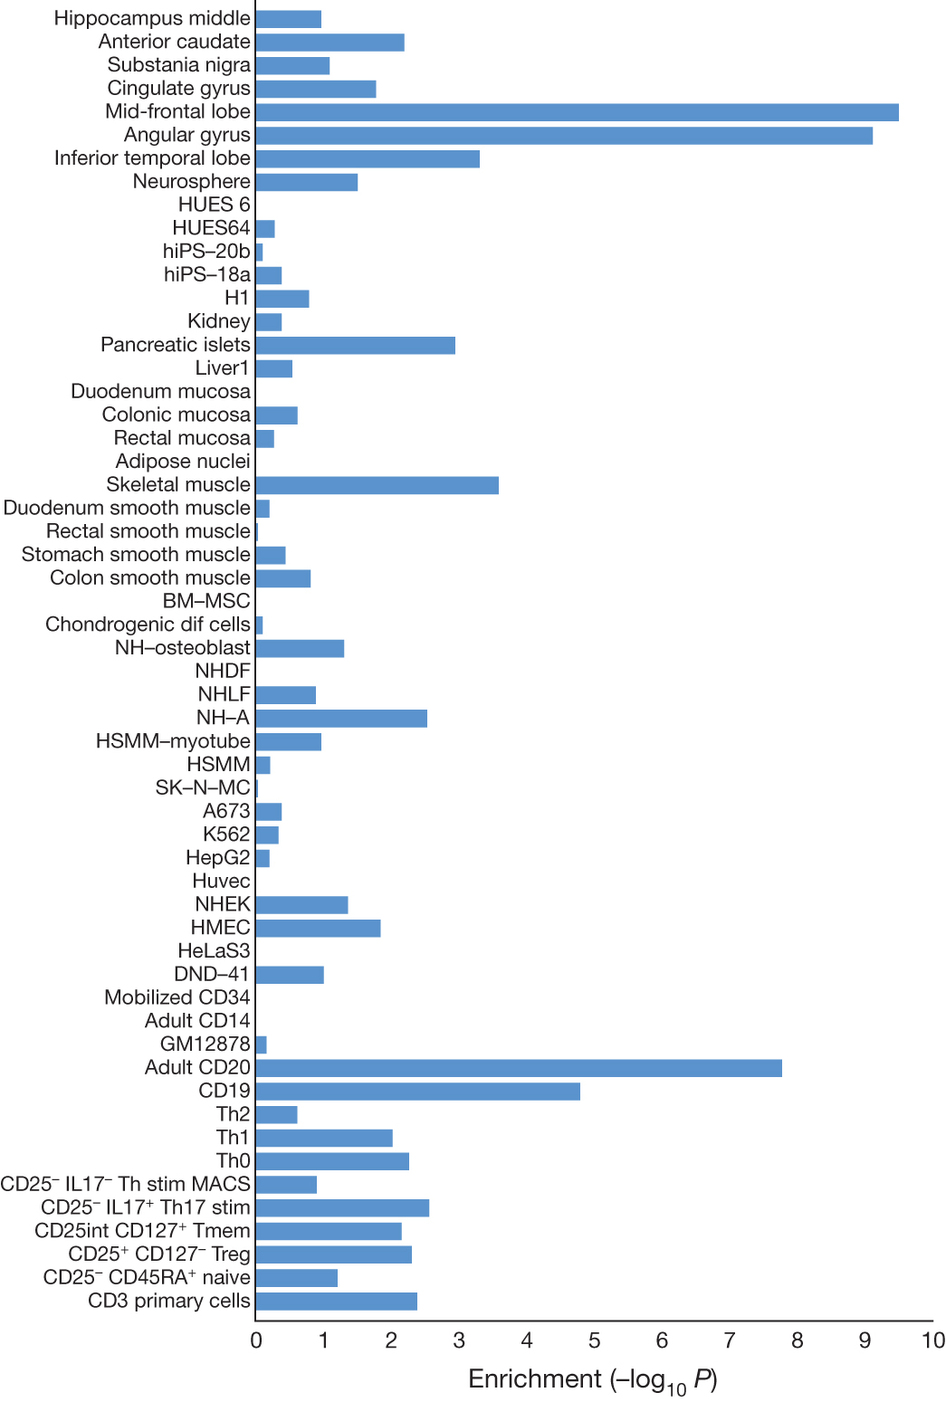
\includegraphics[height=\textwidth]{figure/pgc_enrichment_tissue.jpg}
		\label{fig:pgcEnrich}
	\end{figure}
	It was further demonstrated that \glng{scz} association were significantly enriched at enhancers active in brain and enriched at enhancers active in tissues with important immune functions(\cref{fig:pgcEnrich})\citep{Ripke2014}.
		
	The enrichment of immune related enhancers remains significant even after the removal of \gls{mhc} region from the analysis, provided further genetic support of the involvement of the immune system in the etiology of \glng{scz}.
	Because of its role in neural development\citep{Zhao1998,Deverman2009}, it is likely that the perturbation in the immune system might disrupt the brain development, therefore increasing the risk of \glng{scz}.
	Indeed, studies on \gls{mia} has demonstrated that cytokine imbalance might predispose individual to \glng{scz}\citep{Meyer2009}. 
	
	\subsubsection{Copy Number Variation}
	\glsreset{cnv}
	Another important arm of genetic research in \glng{scz} was to identify \gls{cnv} associated with \glng{scz}.
	\gls{cnv} were classified as segment of DNA that is 1kb or larger and that is present at a different copy number when compared to the reference genome, usually in the form of insertion, deletion or duplication\citep{Feuk2006}.
	Due to the length of these variants, the \gls{cnv} might contain the entire genes and their regulatory regions which might in turn contribute to significant phenotypic differences\citep{Feuk2006}.
	
	To identify robust association between \gls{cnv} and \glng{scz}, \cite{Szatkiewicz2014} conducted a \gls{GWAS} for \gls{cnv} association with \glng{scz} used the Swedish national sample (4,719 \glng{scz} samples and 5,917 controls).
	In their study, they were able to association between \glng{scz} and \gls{cnv} such as 16p11.2 duplications, 22q11.2 deletions, 3q29 deletions and 17q12 duplications were identified.
	Through the gene set association analysis, calcium channel signaling and binding partners of the fragile X mental retardation protein were found to be associated with these \gls{cnv}\citep{Szatkiewicz2014}.
	Interestingly, the calcium channel signaling were also enriched in the \gls{pgc} \gls{GWAS} on \gls{SNP} association, suggesting that the variants were converging on similar set of pathway or gene sets. 
	
	% I need to state rare and large effect because LDSC cannot do that 
	Unlike the result form the \gls{GWAS} on \gls{SNP} data, the \gls{cnv} identified were rare($\le12$ in 4,719 samples) and has a relative large effect (e.g. 22q11 deletion has an odd ratio of 16.32\citep{Szatkiewicz2014}). 
	The results from the \gls{SNP} \gls{GWAS} supports the ``common disease-common variant'' model whereas the \gls{GWAS} on \gls{cnv} supports the ``common disease-rare variant'' model, illustrating the complex genetic model behind the etiology of \glng{scz}.
	
	Although the \gls{GWAS} in \glng{scz} seems to return a lot of interesting results, the question remains: How much of the known genetic risk factors associated explain the disease risk of \glng{scz}?
	To answer these question, we need to estimate the heritability based on the \gls{GWAS} data. 
	However, in order to obtain the large volume of data, most of the samples were not relatives. 
	How can one estimate the heritability based only on the genetic data of the general population instead of family or twin data?
	